% !TeX root = ../libro.tex
% !TeX encoding = utf8

\chapter{Planificación y costes del proyecto}\label{ap:pyc}

Para realizar este trabajo, se ha seguido una planificación guiada a través de un diagrama de Gantt, el cual se puede ver en la Figura \ref{fig:proy}. En este diagrama, exponemos cada una de las fases del proyecto y un tiempo aproximado de cuánto ha durado cada una de ellas. Se empezó con un estudio de los fundamentos de la teoría de códigos, se siguió con la redacción de la memoria y por último, se implementó el código del trabajo.

\begin{figure}[h]
    \centering
    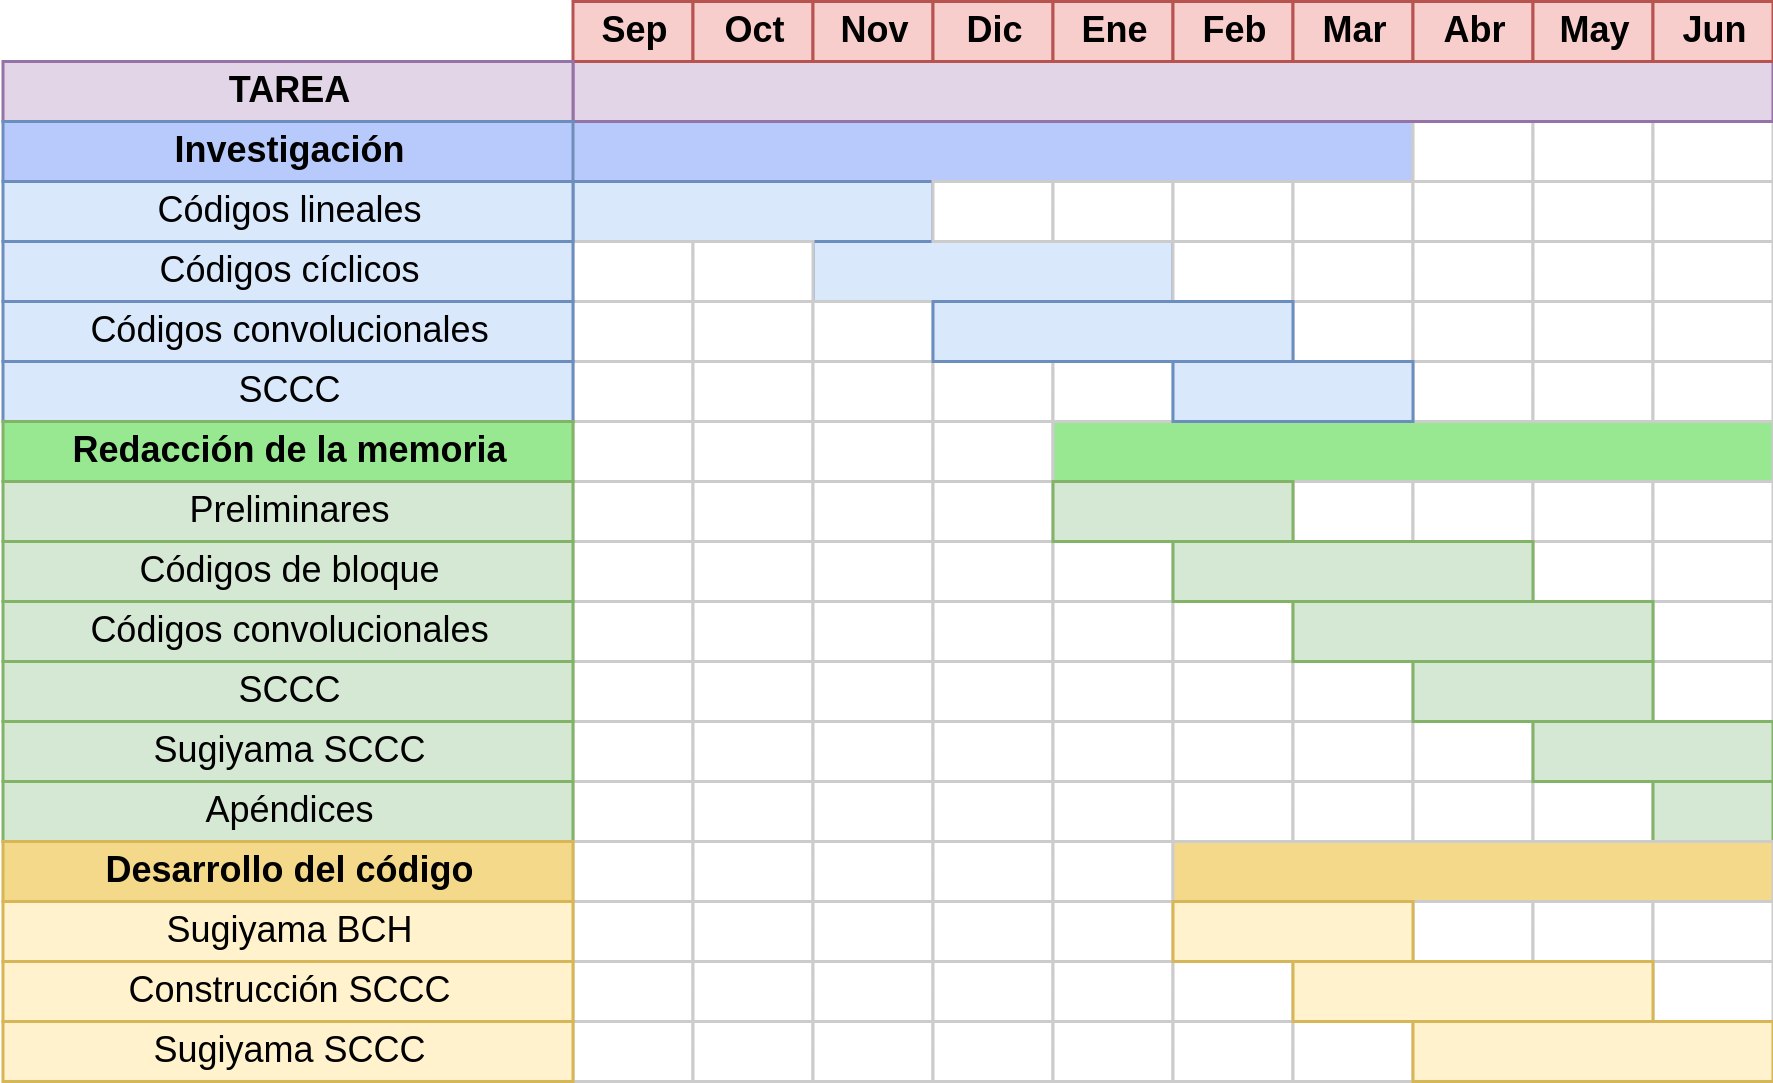
\includegraphics[width=1\textwidth]{img/GRANTT.png}
    \caption{Planificación temporal de las etapas del proyecto.}
    \label{fig:proy}
\end{figure}

\newpage

Vamos a realizar también una aproximación del coste monetario de la creación de este proyecto, considerando su duración de 9 meses. Estos cálculos se realizarán teniendo en cuenta que se han trabajado 450 horas de acuerdo a los 18 créditos ECTS correspondientes asignados al TFG y con un gasto aproximado de 20 €/h.


\begin{small}
    \begin{longtable}{|>{\raggedright\arraybackslash}p{3cm}|>{\raggedright\arraybackslash}p{4cm}|>{\centering\arraybackslash}p{2cm}|>{\centering\arraybackslash}p{2cm}|}
    \hline
    \textbf{Tipo} & \textbf{Tareas} & \textbf{Cantidad (h)} & \textbf{Coste (€)} \\
    \hline
    \endfirsthead
    \hline
    \textbf{Tipo} & \textbf{Tareas} & \textbf{Cantidad (h)} & \textbf{Coste (€)} \\
    \hline
    \endhead
    \hline
    Investigación & Códigos lineales & 30 & 600 \\
    \hline
    Investigación & Códigos cíclicos & 30 & 600 \\
    \hline
    Investigación & Códigos convolucionales & 50 & 1000 \\
    \hline
    Investigación & Códigos convolucionales cíclicos sesgados & 40 & 800 \\
    \hline
    Implementación del código & Sugiyama para BCH & 30 & 600 \\
    \hline
    Implementación del código & Construcción de códigos SCCC & 40 & 800 \\
    \hline
    Implementación del código & Sugiyama para SCCC & 50 & 1000 \\
    \hline
    Redacción de la memoria & Preliminares & 20 & 400 \\
    \hline
    Redacción de la memoria & Códigos de bloque & 50 & 1000 \\
    \hline
    Redacción de la memoria & Códigos convolucionales & 50 & 1000 \\
    \hline
    Redacción de la memoria & SCCC y Sugiyama para SCCC & 60 & 1200 \\
    \hline
    \hline
    \textbf{Total} & & 450 & 9000 \\
    \hline
    \caption{Distribución de tareas y costos}
    \label{tab:costos}
    \end{longtable}
\end{small}
    
La Tabla \ref{tab:costos} se puede observar cuánto tiempo ha requerido cada tarea junto al coste total calculado.

\endinput
